\renewcommand{\reqid}{N/A}
\renewcommand{\procid}{SB1FS-COM-F-012}
\renewcommand{\procname}{Aliveness and Functional Test\xspace}

\section{\procid \ \procname} \label{sec:SB1FS-COM-F-012}
\begin{table}[H]
	\centering
	\footnotesize
	\begin{tabular}{|L{3.0cm}|L{13.0cm}|}	
		%\hline
		%\textbf{Requirement ID} 	& \reqid\\
		%\hline
		%\textbf{Requirement Statement} & N/A\\
		\hline
		\textbf{Task ID} & \procid \\
		\hline
		\textbf{Task name} & \procname \\
		\hline
		\textbf{Task description} & In this procedure the EWC30 X-Band transmitter functional test is performed.
		
		First of all, CEGSE interfaces aliveness is performed,
  Transmitter and Filter ground connections are verified and 
   RF and base-band DUT interfaces are connected to EGSEs.
   DUT monitoring and control is performed from CEGSE{}.
  Oscilloscope and PXI spectrum analyzer are configured 
  to measure power consumption and RF signals characteristics respectively.
Data frames will be sent from CEGSE to  EWC30 in order to be modulated through X-Band interface. 
 The data received in \fmr{} will be compared with 
 original data.\\
		\hline
		\textbf{Task purpose} & Execution of EWC30 functional test. \\
		\hline
		\textbf{Success criteria} & 			\begin{minipage}[t]{\linewidth}
			\begin{itemize}[nosep,after=\strut]
		\item CEGSE and \fmr{}, are configured according to procedure and CEGSE interfaces are in good condition.
DUT telemetry is between expected values.
	\item Measurements of voltages, currents and power consumptions in different states meets the expected values.
	\item RF signals are under expected values.
	\item Data frames received at GS-GSE are the same as those sent from CEGSE.
	\item Evidences are collected. 
				\end{itemize}
		\end{minipage}\\
		\hline
		\textbf{Test sub-cases} & 
\begin{minipage}[t]{\linewidth}
		\begin{itemize}[nosep,after=\strut]
		\item \procid{-01}: Test setup and configuration
		\item \procid{-02}: Inrush and ripple measurement 
		\item \procid{-03}: Aliveness and Functional Test
		\item \procid{-04}: Tests setup break
		\end{itemize}
		\end{minipage}\\
		\hline
		\textbf{Test Setup} &
\begin{minipage}[t]{\linewidth}
	\begin{itemize}[nosep,after=\strut]
		\item \comEgse\xspace to DUT base-band electrical connections according to figures \ref{fig:ewc30_bb_ripple} and \ref{fig:ewc30_bb} 
		\item General setup according to figure \ref{fig:setup_xband_funcional_ripple} for inrush and ripple measurements. Figure \ref{fig:setup_xband_funcional} for Data Downlink test.
		\end{itemize}
	\end{minipage}	
		\\ 
		\hline
		\textbf{Duration} & \begin{minipage}[t]{\linewidth}
	\begin{itemize}[nosep,after=\strut]
		\item \procid{-01}: 150 minutes
		\item \procid{-02}: 150 minutes \tr{actulizar}

		\item \procid{-03}: 180 minutes \tr{actulizar}		
		\item \procid{-04}: 45 minutes 
		\end{itemize}
	\end{minipage}
	\\ \hline
	
	\textbf{Data sets required} &  \begin{minipage}[t]{\linewidth}
		\begin{itemize}[nosep,after=\strut]
			%\item Data payload file to send (\texttt{Data-885840\_120s\_IDLE\_VCh01\_IDLE\_sent.bin}).
			\item Payload file (\texttt{Data-885840\_120s\_VCh01\_payload.bin})
			\item \comEgse\xspace PXI configuration file for aliveness (\texttt{INIT\_FILE\_NO\_ALARM\_EWC30.ini}).
			\item \comEgse\xspace PXI nominal configuration file for EWC30 (\texttt{INIT\_FILE\_EWC30.ini}).
			%\item Oscilloscope configuration files in \texttt{osc-config} folder
			\item PXI spectrum analyzer configuration file in \texttt{NI-RFSA-data-config} folder
			%\item \texttt{SB1-Data-VC63-10minutes.zip} file
			%\item GS-GSE M\&C scripts (\texttt{gse\_const.py, gse\_mandc.py, SB1GS-GSE-EM2.0-DemoData-RF-N1.py})
				\end{itemize}
			\end{minipage}\\
		\hline
		
				\textbf{Prerequisites} & 
		\begin{minipage}[t]{\linewidth}
			\begin{itemize}[nosep,after=\strut] 
				%\item GS-GSE-FM (R) initialized according to GS-GSE test procedures (\refAD{fm-ver-delta-pro}) or  user manual (\refRD{gs-gse-fm}). 
				%\item GS-GSE-FM (R) configured according to Control Configuration Documents (\refAD{gse-cfg-r}) and modified according to report (\refAD{reportFMRMod}).
 	%\item \comEgse initialized according to \comEgse\xspace user manual (\refAD{cegse}).
				\item Execution of procedure SB1FS-COM-D-011 Initialization and dataset deploy.
				\item EWC30 and DSN filter mated with the connector savers (RF and BB).
				\item EWC30 and DSN filter mounted on \comEgse\xspace metal tray.
				\item EWC30 and DSN filter connected to grounding bar.
				\item Hardware: The necessary items are shown in the table \ref{tab:req-items} 
			\end{itemize} 
		\end{minipage}\\
		\hline
		
	\end{tabular}
	\caption{Procedure \procid \ description. } \label{tb:\procid-001}
\end{table}

\begin{comment}%%%%%%%%%%%%
\begin{figure}[H]
	\centering
	\includegraphics[height=11.5cm]{figuras/DSN_Setup.png} 
	\caption{\procid \ Test setup for X-Band DSN filter characterization.}
	\label{fig:DSN_setup}
\end{figure}

\begin{figure}[H]
	\centering
	\includegraphics[width=0.75\linewidth]{figuras/setup.jpg}  
	\caption{\procid \  representation picture of test setup for X-Band DSN filter.}
	\label{fig:foto}
\end{figure}

\begin{table}[H]
	\centering
	\includegraphics[width=0.75\linewidth]{figuras/pass_fails.jpg}  
	\caption{\procid \ X-Band DSN filter characterization Pass/fails criteria.}
	\label{fig:pass_fails}
\end{table}
\end{comment}


%% Test Setup
\begin{figure}[H]
	\centering
	  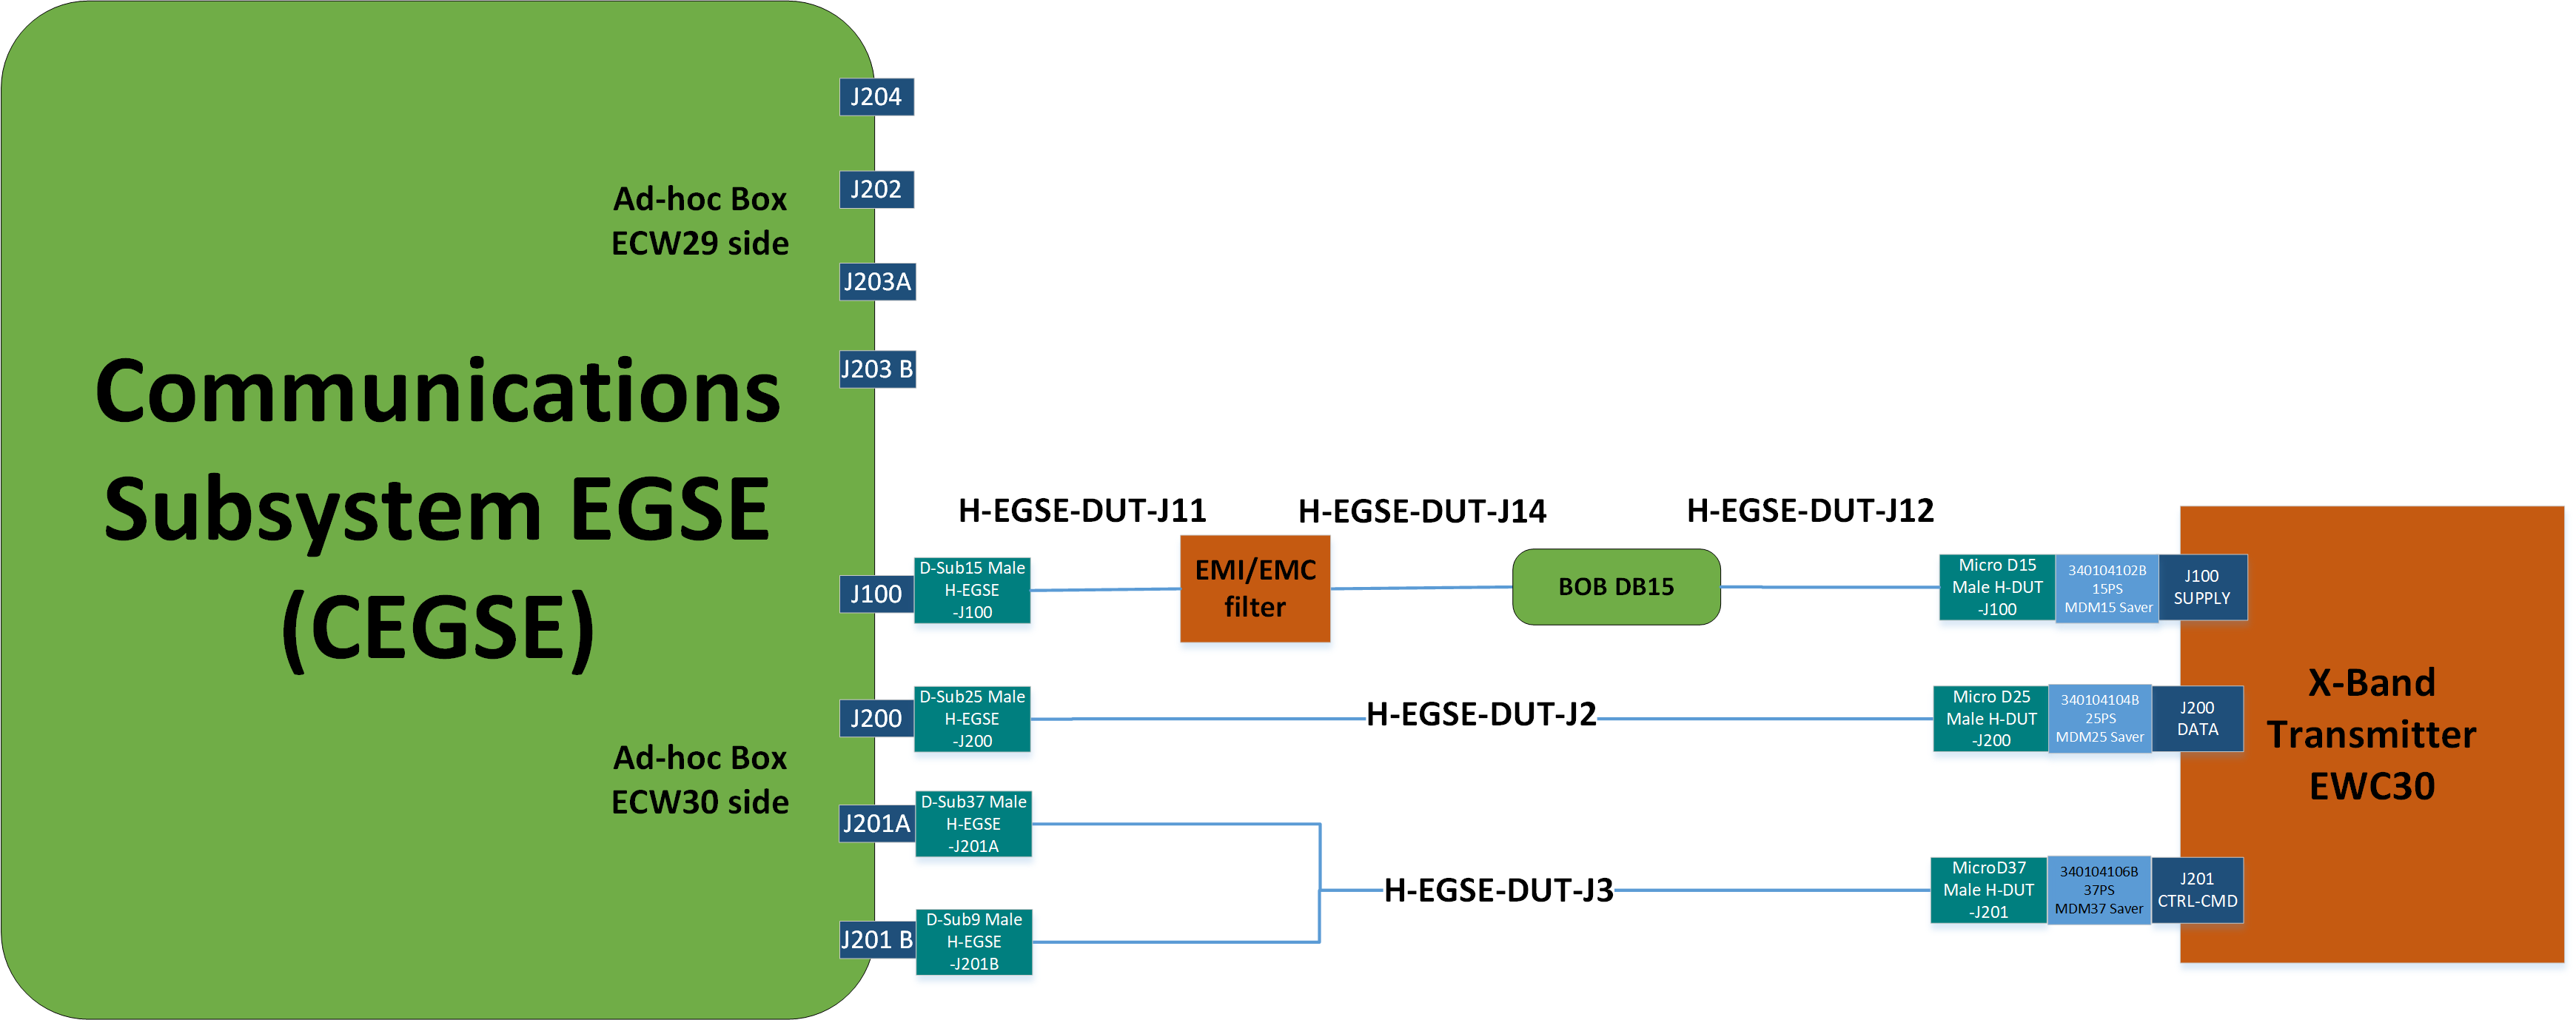
\includegraphics[width=.9\linewidth]{figuras/CEGSE_EWC30SetupA.png}  
	  \caption{EWC-30 BB connections for inrush and ripple measurement.}
	\label{fig:ewc30_bb_ripple}
\end{figure}

%% Test Setup
\begin{figure}[H]
	\centering
	  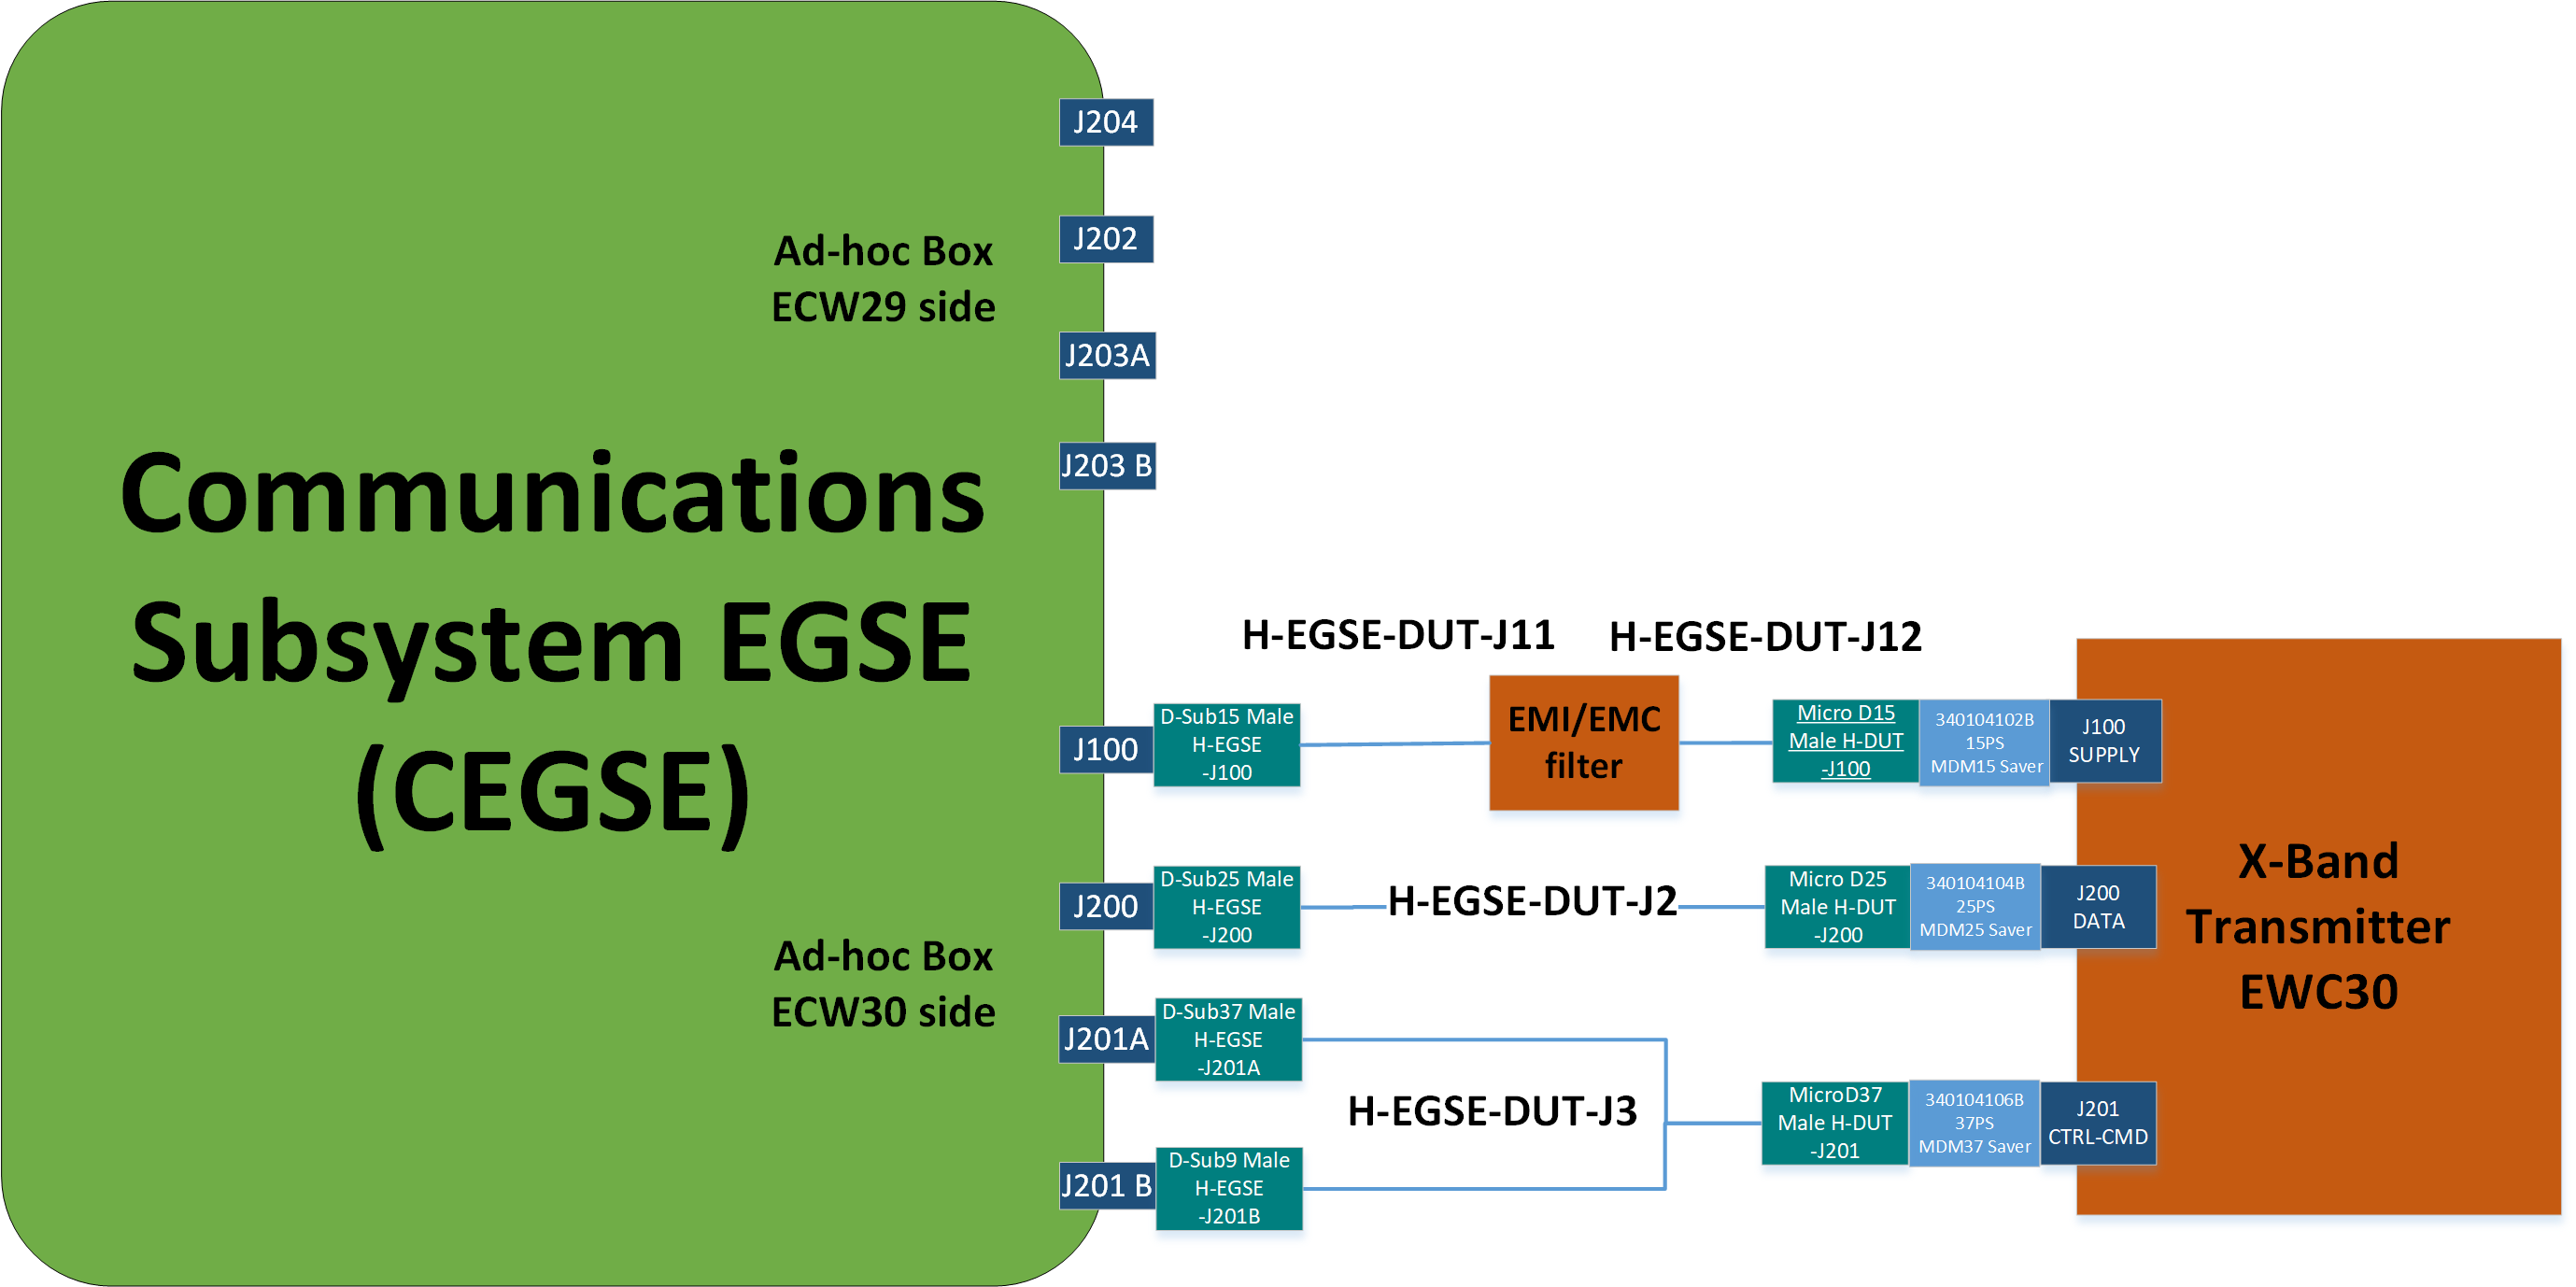
\includegraphics[width=.7\linewidth]{figuras/CEGSE_EWC30SetupB.png}  
	  \caption{EWC-30 BB general connections.}
	\label{fig:ewc30_bb}
\end{figure}

